\documentclass[t, screen, aspectratio=43]{beamer}
\usepackage[T1]{fontenc}
\usepackage[utf8]{inputenc}
\usepackage{epsf}
\usepackage{graphicx}
\usepackage{geometry}
\usepackage{tabularx}
\usepackage[table]{colortbl}
\usepackage{xcolor}
\usepackage{soul}
\usepackage[normalem]{ulem}
\usepackage{tikz}
\usepackage{subcaption}
% Use the NTNU-temaet for beamer 
% \usetheme[style=ntnu|simple|vertical|horizontal, 
%     language=bm|nn|en, 
%     smalltitle, 
%     city=all|trondheim|alesund|gjovik]{ntnu2017}
\usetheme[style=helvet,language=en]{ntnu2017}

\usepackage[english]{babel}
\usepackage[style=numeric,backend=biber,natbib=false,sorting=none]{biblatex}

\title[Short title]{Python Framework for Design and Analysis of Integer-N ADPLLs}
\subtitle{Specialization Project Progress - 13th Week}
\author[C Nielsen]{Cole Nielsen}
\institute[NTNU]{Department of Electronic Systems, NTNU}
\date{22 November 2019 (Calendar week 47)}
%\date{} % To have an empty date

\addbibresource{example.bib} % Add bibliography database

% Set the reference style to numeric.
% See here: http://tex.stackexchange.com/questions/68080/beamer-bibliography-icon
\setbeamertemplate{bibliography item}[text] 

% Set bibliography fonts to a small size.
\renewcommand*{\bibfont}{\footnotesize}




\begin{document}

\begin{frame}
	\titlepage%
\end{frame}

% Alternatively, special title page command to get a different background
% \ntnutitlepage

% #############################################################################
% Timeline
% #############################################################################

\begin{frame}
	\frametitle{Timeline}
	\begin{table}[htb!]
		\tiny
		\centering
		\vspace{-1em}
		\def\arraystretch{1.5}		
		\setlength\arrayrulewidth{0.75pt}
		\setlength{\tabcolsep}{1em} % for the horizontal padding
		\begin{tabular}{|l|l|l|l|}
			\hline 
			\rule[-1ex]{0pt}{2.5ex} \cellcolor{gray!40}\textbf{Week} & \cellcolor{gray!40}\textbf{Dates} &\cellcolor{gray!40}\textbf{Tasks} & \cellcolor{gray!40}\textbf{Outcomes}\\ 
			\hline 
			\rule[-1ex]{0pt}{2.5ex} \cellcolor{red!20}\textbf{36}& \cellcolor{red!20}2.9 - 8.9 & \cellcolor{red!20}Review PLL Design & \cellcolor{red!20}Refreshed Knowledge\\ 
			\hline 
			\rule[-1ex]{0pt}{2.5ex} \cellcolor{red!20}\textbf{37}& \cellcolor{red!20}9.9 - 15.9 & \cellcolor{red!20}Modeling/simulation (set up) & \cellcolor{red!20}--\\ 
			\hline 
			\rule[-1ex]{0pt}{2.5ex} \cellcolor{red!20}\textbf{38}& \cellcolor{red!20}16.9 - 22.9 & \cellcolor{red!20}Modeling/simulation &\cellcolor{red!20}TDC/DCO Requirements\\ 
			\hline 
			\rule[-1ex]{0pt}{2.5ex} \cellcolor{red!20}\textbf{39}& \cellcolor{red!20}23.9 - 29.9& \cellcolor{red!20}Modeling/simulation& \cellcolor{red!20}Loop Filter/Digital Algorithms\\ 
			\hline 
			\rule[-1ex]{0pt}{2.5ex} \cellcolor{red!20}\textbf{40}& \cellcolor{red!20}30.9 - 6.10& \cellcolor{red!20}Modeling/simulation& \cellcolor{red!20}{Loop filter, DCO, TDC, calibration}\color{black}\\ 
			\hline 
			\rule[-1ex]{0pt}{2.5ex} \cellcolor{red!20}\textbf{41}&\cellcolor{red!20}7.10 - 13.10&\cellcolor{red!20}Circuit Research &\cellcolor{red!20}DCO/Divider topologies\\ 
			\hline 
			\rule[-1ex]{0pt}{2.5ex} \cellcolor{red!20}\textbf{42}&\cellcolor{red!20}14.10 - 20.10&\cellcolor{red!20}Circuit Research &\cellcolor{red!20}TDC/other topologies\\ 
			\hline 
			\rule[-1ex]{0pt}{2.5ex} \cellcolor{red!20}\textbf{43}&\cellcolor{red!20}21.10 - 27.10&\cellcolor{red!20}Spur analysis, filter automation &\cellcolor{red!20} \\ 
			\hline 
			\rule[-1ex]{0pt}{2.5ex} \cellcolor{red!20}\textbf{44}&\cellcolor{red!20}28.10 - 3.11&\cellcolor{red!20}Filter automation, SNR estimation&\cellcolor{red!20}\\ 
			\hline 
			\rule[-1ex]{0pt}{2.5ex} \cellcolor{red!20}\textbf{45}&\cellcolor{red!20}4.11 - 10.11&\cellcolor{red!20}Variation analysis, flicker noise &\cellcolor{red!20}Histograms/yield estimates\\ 
			\hline 
			\rule[-1ex]{0pt}{2.5ex} \cellcolor{red!20}\textbf{46}&\cellcolor{red!20}11.11 - 17.11&\cellcolor{red!20}Real DCO sensitivity, TDC/divider jitter&\cellcolor{red!20}Simlate ring-DCO in Virtuoso\\ 
			\hline 
			\rule[-1ex]{0pt}{2.5ex} \cellcolor{green!20}\textbf{47}&\cellcolor{green!20}18.11 - 24.11&\cellcolor{green!20}{\color{red}\st{PLL + Radio simulation} }{\color{blue}\textbf{Report}}&\cellcolor{green!20}\color{red}{\st{BER estimate}}\\ 
			\hline 
			\rule[-1ex]{0pt}{2.5ex} \textbf{48}& 25.11 - 1.12& Organize code, Report & (I have an Exam on 30.11)\\ 
			\hline 
			\rule[-1ex]{0pt}{2.5ex} \textbf{49}& 2.12 - 8.12& {\color{blue}\textbf{PLL/Radio BER simulation}}, Report& \\ 
			\hline 
			\rule[-1ex]{0pt}{2.5ex} \textbf{50}& 9.12 - 15.12& Report writing& Complete by 14.12\\ 
			\hline 
		\end{tabular}
		\begin{flushleft}\textbf{Legend:} \colorbox{red!20}{\textbf{Done}} \colorbox{green!20}{\textbf{Current}}  \colorbox{blue!20}{\textbf{Revised}}
		% *I will write the report simultaneously with the work.
		\end{flushleft}
		% \caption{Assigned specifications for branch line hybrid design.}
		% \label{asgn_specs}
	\end{table}   
\end{frame}


% #############################################################################
% This week
% #############################################################################

\begin{frame}
	\frametitle{Timeline Tasks}
	\begin{block}{This week}
		\begin{itemize}
			\footnotesize
			\item \textbf{Report writing}
			\begin{itemize}
				\footnotesize
				\item Redirected focus this week to writing as it is high priority.
			\end{itemize} 
			\item {\color{red}\textbf{PLL/Radio BER simulation}}
			\begin{itemize}
				\footnotesize
				\item Original plan for week. Less of a priority, moved to after 30 November (post-exams for me).
			\end{itemize} 
			\item \textbf{Ring oscillator simulation in 22FDX:}
			\begin{itemize}
				\footnotesize
				\item Fit simulation data to model, reasonably accurate.
				\item Not sure this fits in well with the report.
			\end{itemize} 
		\end{itemize}    
	\end{block}
\end{frame}

% #############################################################################
% sim/modeling approach
% #############################################################################

\begin{frame}
	\frametitle{Report writing}
	\begin{block}{Format}
			%\center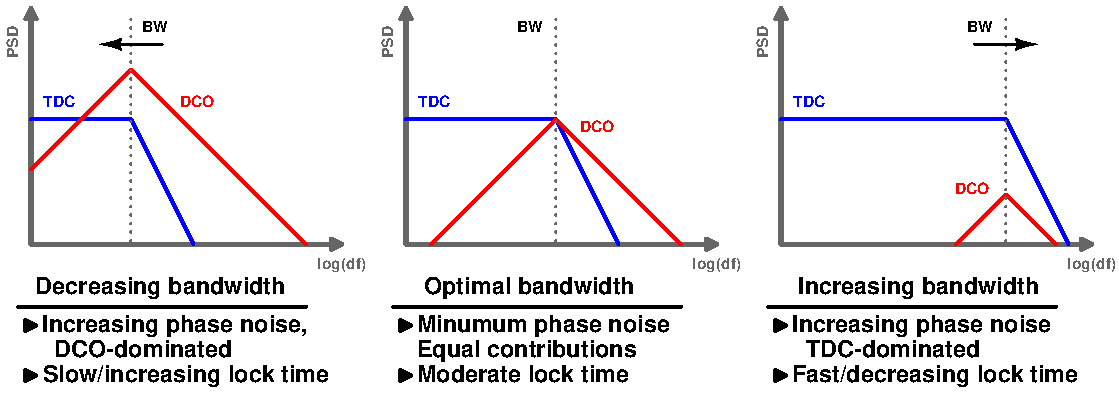
\includegraphics[width=0.8\textwidth, angle=0]{loop_bandwidth.pdf}
		\begin{itemize}
			\scriptsize
			\item Abstract
			\item Problem/project description
			\item Introduction
			\item Theory
			\begin{itemize}
				\scriptsize
				\item Discuss theory relevant to understand the simulation engine and optimizer.
			\end{itemize}
			\item Methods
			\begin{itemize}
				\scriptsize
				\item Describes how the simulator is implemented, how the filter designer/optimizer is implemented.
			\end{itemize}
			\item Discussion (combined with results)
			\begin{itemize}
				\scriptsize 
				\item Discuss choices made in simulator/optimizer design, compare to existing solutions, design examples
			\end{itemize}
			\item Concusion
		\end{itemize}    
	\end{block}
\end{frame}

\begin{frame}
	\frametitle{Report writing}
	\begin{block}{Theory section}
			%\center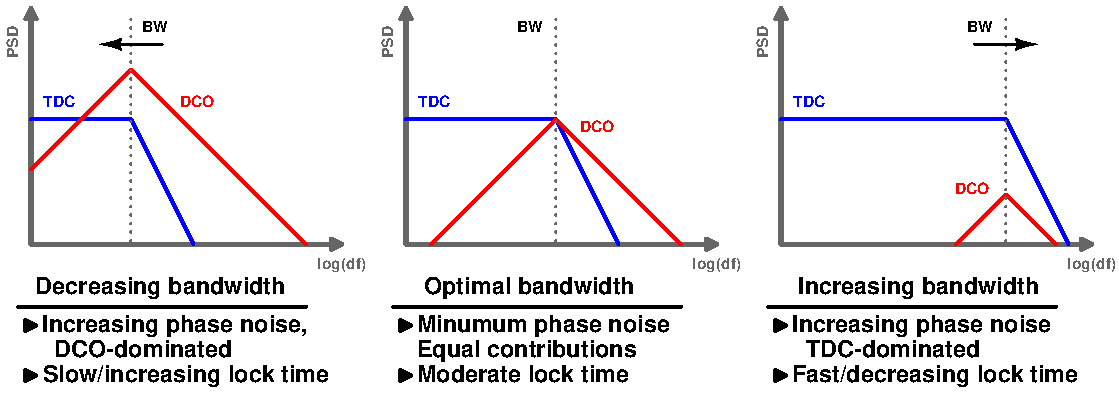
\includegraphics[width=0.8\textwidth, angle=0]{loop_bandwidth.pdf}
		\begin{itemize}
			\scriptsize
			\item Introduce what a PLL is
			\item Develop basic fully continuous PLL model
			\begin{itemize}
				\scriptsize
				\item Use continuous model to develop basic PI-continuous loop filter.
			\end{itemize}
			\item Develop discrete-time, digital PLL model from continuous model
			\begin{itemize}
				\scriptsize
				\item Both the discrete transfer-function and continous approximations developed.
			\end{itemize}
			\item Pll phase noise
			\begin{itemize}
				\scriptsize 
				\item Derive/explain basic phase noise models for all PLL components
				\item Derive PLL noise PSD from PLL phase signal
				\item Derive PLL noise sensitivity functions
			\end{itemize}
		\end{itemize}    
	\end{block}
\end{frame}

\begin{frame}
	\frametitle{Report writing}
	\begin{block}{Methods}
			%\center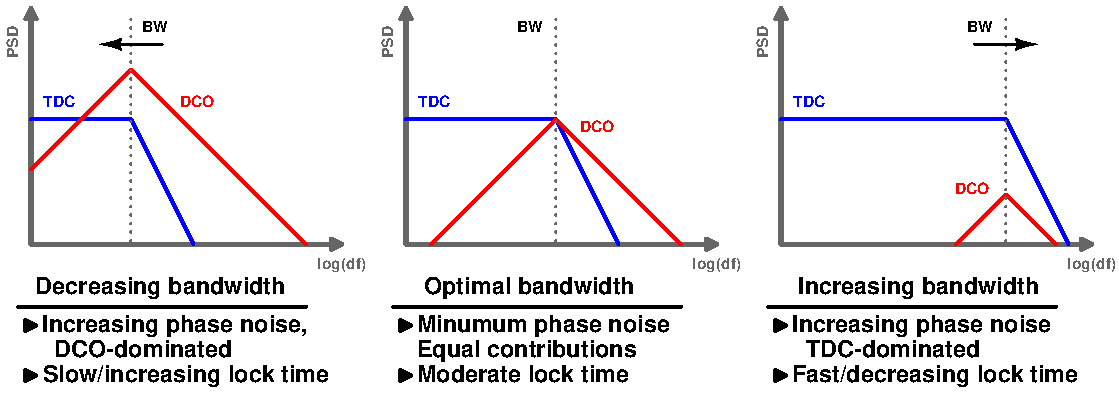
\includegraphics[width=0.8\textwidth, angle=0]{loop_bandwidth.pdf}
		\begin{itemize}
			\scriptsize
			\item Simulator implementation
			\begin{itemize}
				\scriptsize
				\item Describe how to implement a accurate oscillator phase noise in discrete time simulation
				\item Describe discrete phase noise/spur measurement simulation requirements and calculation method
				\item Describe Monte-Carlo sampling engine
			\end{itemize}
			\item Optimizer implementation
			\begin{itemize}
				\scriptsize
				\item Describe implementation of fast settling time and phase noise estimation heuristics
				\item Describe loop filter optimizer algorithm to perform phase noise minimization with constrained settling time
				\item Describe second order optimization of loop filter implementation resolution.
				\item Describe BER simulation implementation.
			\end{itemize}
		\end{itemize}    
	\end{block}
\end{frame}

\begin{frame}
	\frametitle{Report writing}
	\begin{block}{Discussion}
			%\center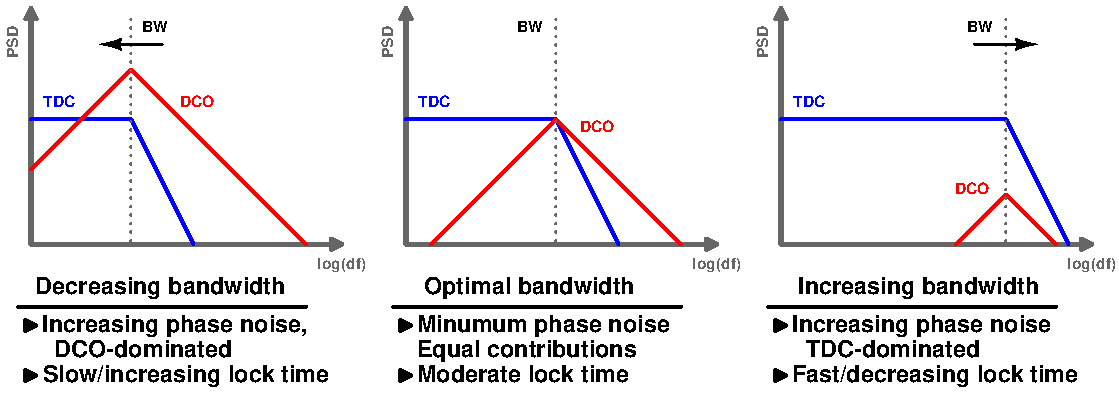
\includegraphics[width=0.8\textwidth, angle=0]{loop_bandwidth.pdf}
		\begin{itemize}
			\scriptsize
			\item Simulator/optimizer implementation
			\begin{itemize}
				\scriptsize
				\item Discuss choices made in simulator/optimizer approach
			\end{itemize}
			\item Comparison to existing solutions
			\begin{itemize}
				\scriptsize
				\item Discuss what has been done before, what is new with this approach, compare performance?
			\end{itemize}
			\item Design example
			\begin{itemize}
				\scriptsize
				\item Show design process and results (simulation) with engine
				\item Mention any considerations that must be made using the engine (i.e. pitfalls)
			\end{itemize}
		\end{itemize}    
	\end{block}
\end{frame}



\begin{frame}
	\frametitle{Ring oscillator in 22FDX}
	\begin{block}{Ring oscillator model fit}
			%\center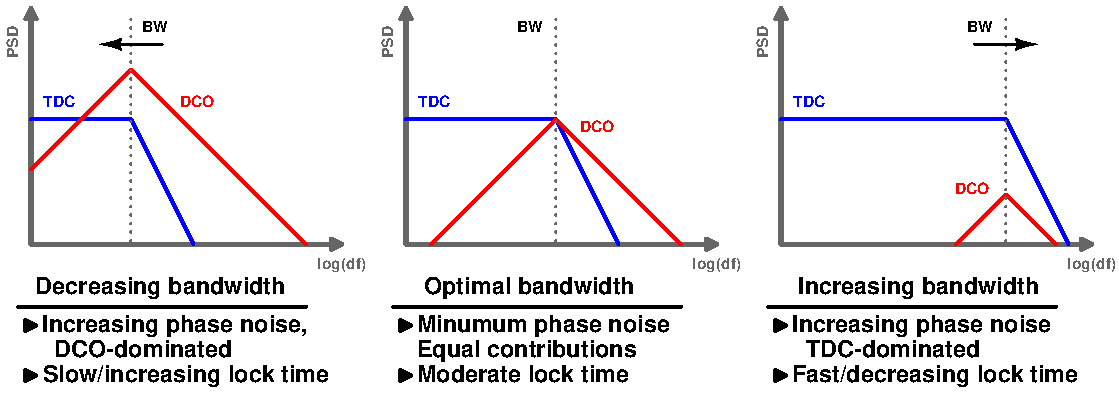
\includegraphics[width=0.8\textwidth, angle=0]{loop_bandwidth.pdf}
	\scriptsize
	\begin{itemize}
		\item Last week discussed simulation of ring oscillator
		\item Curve fitted the below equation based on the following parameter sweeps: RVT/SLVT devices, varied temp in \{-40, 25, 85\}, L in \{100n, 500n\}, W/L in \{1, 10\}, $C_{load}$ in \{0, 1f, 10f\}, $V_{BB}$ in \{0, 0.8\}
		\item Now have estimates for model of $\mu_n$, $C_ox$, body effect coefficient $\gamma$ and $V_{t0}$
	\end{itemize}
	\begin{equation}
		f_{osc} = \frac{\mu_nC_{ox}}{4\ln2NC}\left(\frac{W}{L}\right)_n\left[V_{DD}\left(\frac{7}{8\ln2}-1\right)-V_{t0}\left(\frac{1}{\ln2}-1\right) + \gamma V_{BG}\left(\frac{1}{\ln2}-1\right) \right]
	\end{equation}
	Via the Python simulation, can apply Monte-Carlo sampling to these model parameters to capture effects of variation of DCO gain:
	\begin{equation}
		\frac{\partial f_{osc}}{\partial V_{BG}} = \gamma V_{BG}\frac{\mu_nC_{ox}}{4\ln2NC}\left(\frac{W}{L}\right)_n\left[\frac{1}{\ln2}-1\right]
	\end{equation}	  
	\end{block}
\end{frame}

\begin{frame}
	\frametitle{Ring oscillator in 22FDX}
	\begin{block}{Ring oscillator model - fitted parameters}
			%\center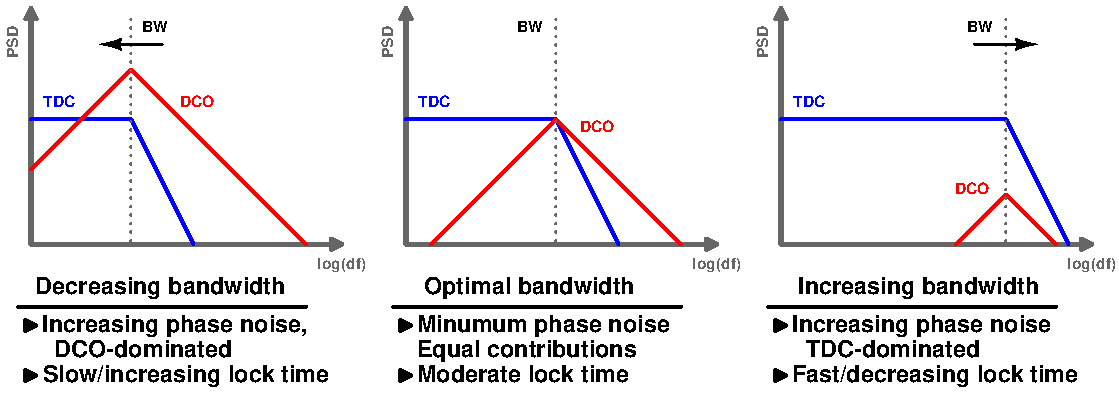
\includegraphics[width=0.8\textwidth, angle=0]{loop_bandwidth.pdf}  
		\begin{table}[htb!]
			\tiny
			\centering
			\def\arraystretch{1.5}		
			\setlength\arrayrulewidth{0.75pt}
			\setlength{\tabcolsep}{1em} % for the horizontal padding
			\begin{tabular}{|l|l|l|l|l|}
				\hline 
				\rule[-1ex]{0pt}{2.5ex} \cellcolor{gray!40}\textbf{Parameter} & \cellcolor{gray!40}\textbf{NFET} & \cellcolor{gray!40}\textbf{SLVTNFET}& \cellcolor{gray!40}\textbf{PFET} & \cellcolor{gray!40}\textbf{SLVTPFET} \\ 
				\hline 
				\rule[-1ex]{0pt}{2.5ex} $V_{th}$ [mV] & 390-0.69T & 340-0.67T & -387+0.88T & -312+0.77T\\ 
				\hline 
				\rule[-1ex]{0pt}{2.5ex} $\gamma $ [V/V]  & -0.072 & -0.083 & 0.082 & 0.069\\ 
				\hline 
			\end{tabular} 
			% \caption{Assigned specifications for branch line hybrid design.}
			% \label{asgn_specs}
		\end{table}  
		\center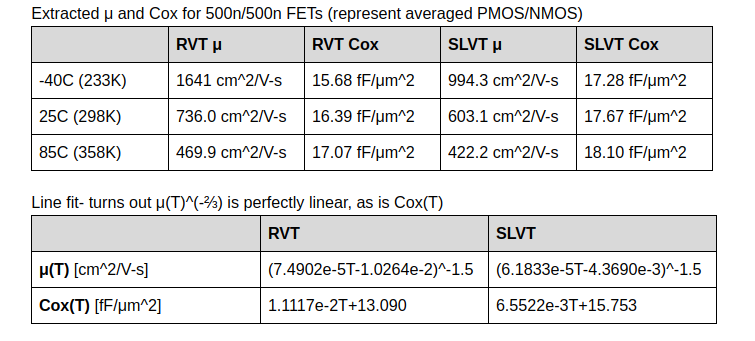
\includegraphics[width=0.7\linewidth]{ro_model_fit.png}
	\end{block}
\end{frame}

\begin{frame}
	\frametitle{Ring oscillator in 22FDX}
	\begin{block}{Include in report???}
			%\center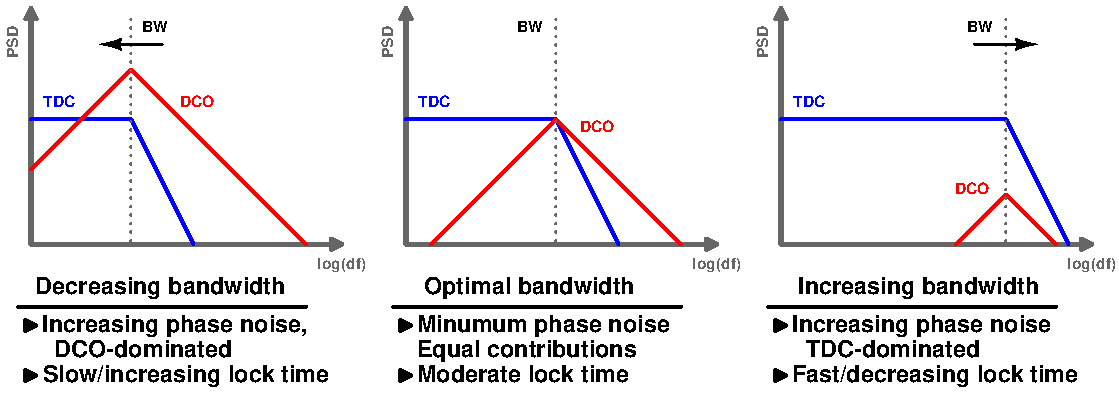
\includegraphics[width=0.8\textwidth, angle=0]{loop_bandwidth.pdf}
		\begin{itemize}
			\scriptsize
			\item Current report is relatively agnostic to implementation. Should this be included as it is a very implementation specific thing?
			\item Perhaps can reserve for later portion of project.
		\end{itemize}    
	\end{block}
\end{frame}


\begin{frame}
	\frametitle{Ring oscillator in 22FDX}
	\begin{block}{Ring oscillator simulation - variation}
			%\center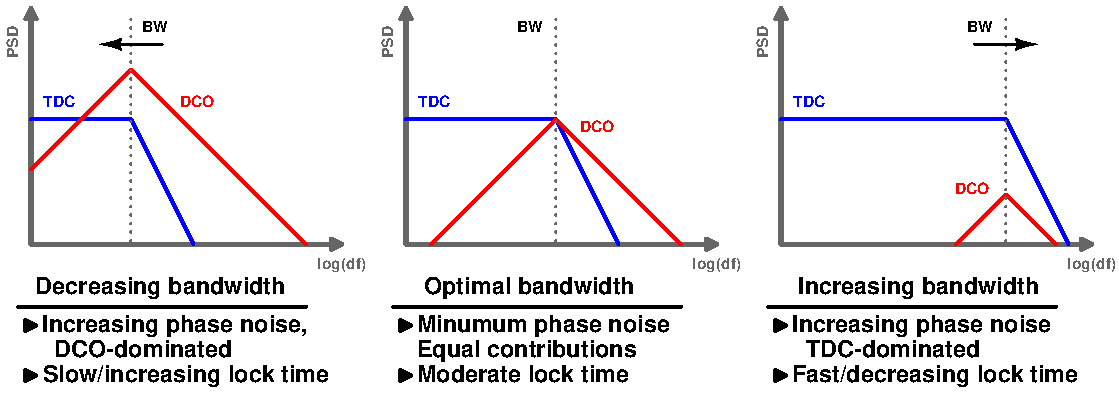
\includegraphics[width=0.8\textwidth, angle=0]{loop_bandwidth.pdf}
		\begin{itemize}
			\scriptsize
			\item Simulated simple 5 stage ring oscillator with $V_{DD}$ = 0.8.
			\item Used RVT/SLVT devices, varied temp in \{-40, 25, 85\}, L in \{100n, 500n\}, W/L in: \{1, 10\}, $C_{load}$ in \{0, 1f, 10f\}, $V_{BB}$ in \{0, 0.8\}
			\item Also perfomed Monte-Carlo at 25C with L=500nm and W/L=1:
			\item Standard deviation for RVT is 4.7\% of nominal value, for SLVT it is 4.5\% of nominal.
		\end{itemize}    
		\center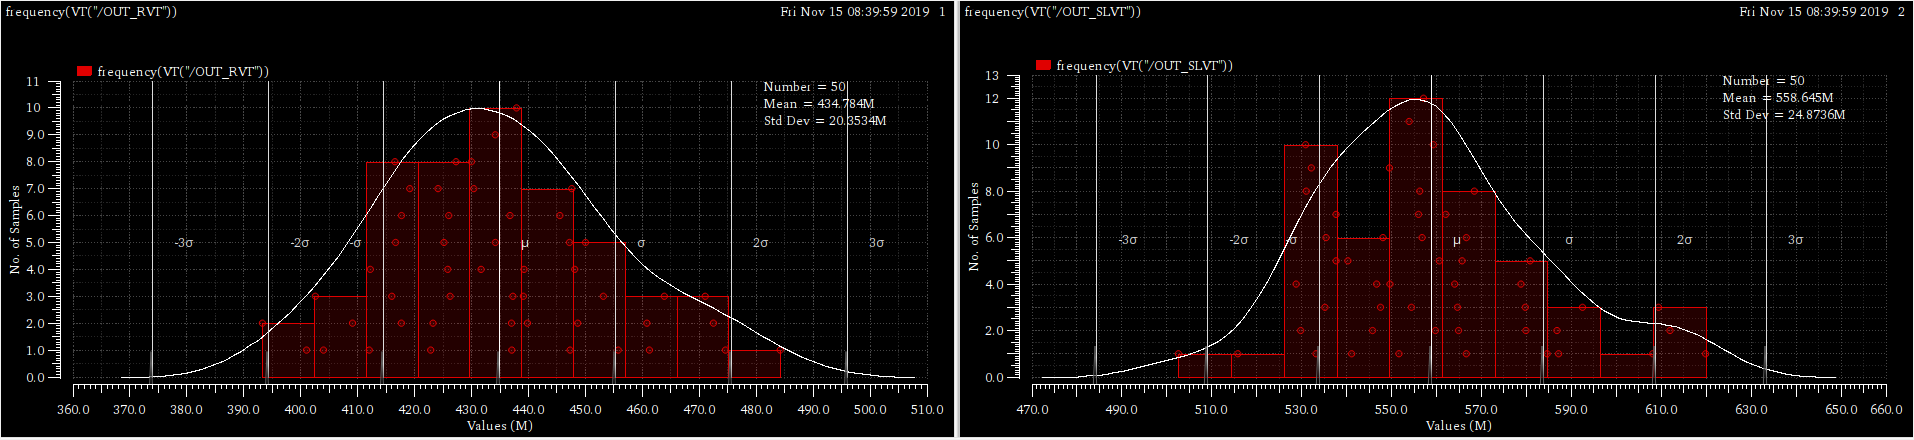
\includegraphics[width=0.8\linewidth]{freq_var.png}
	\end{block}
\end{frame}






% #############################################################################
% Loop Dynamics (continuous)
% #############################################################################

% \begin{frame}
% 	\frametitle{Loop Dynamics}
% 	\begin{block}{Still To Do}
% 		\vspace{-.2em}
% 		\begin{itemize}
% 			\footnotesize
% 			\item Standard approach to used mixed continuous/discrete time mathematical model for DPLL. 
% 			\item Plot of RO phase noise (typical)
% 			\item Automatic analysis of performance (lock detection, residual phase modulation, lock-in/pull-in range).
% 			\item Automatic optimization (using gradient descent) of PLL parameters?
% 			\item Z-domain modeling of loop? Develop (by hand) some ideal transfer funtions for loop.

% 		\end{itemize}    
% 	\end{block}
% \end{frame}

% #############################################################################
% Specification
% #############################################################################

\begin{frame}
	\frametitle{Specification (unchanged)\color{black}}
	\begin{block}{System Performance Targets}
		\scriptsize
		\begin{table}[h!]
			\centering
			\def\arraystretch{1.5}		
			\setlength\arrayrulewidth{0.75pt}
			\setlength{\tabcolsep}{1em} % for the horizontal padding
			\begin{tabular}{|l|r|l|l|}
				\hline 
				\rule[-1ex]{0pt}{2.5ex} \cellcolor{gray!40}\textbf{Parameter} & \cellcolor{gray!40}\textbf{Value} & \cellcolor{gray!40}\textbf{Unit }& \cellcolor{gray!40}\textbf{Notes}\\ 
				\hline 
				\rule[-1ex]{0pt}{2.5ex} \textbf{Frequency}  & 2.4-2.4835 & GHz & 2.4G ISM Band\\ 
				\hline 
				\rule[-1ex]{0pt}{2.5ex} \textbf{Ref. frequency} & 16 & MHz & Yields 6 channels \\ 
				\hline 
				\rule[-1ex]{0pt}{2.5ex} \textbf{Power} & $\leq$ 100  &$\mu$W & \\ 
				\hline 
				\rule[-1ex]{0pt}{2.5ex} \textbf{FSK BER} & $\leq$ 1e-2  & & 2FSK with $f_{dev}$=$\pm$250 KHz\\ 
				\hline 
				\rule[-1ex]{0pt}{2.5ex} \textbf{Initial Lock Time} & $\leq$ 50 & $\mu$s & Upon cold start \\ 
				\hline 
				\rule[-1ex]{0pt}{2.5ex} \textbf{Re-lock Time} & $\leq$ 5 & $\mu$s & Coming out of standby \\ 
				\hline 
				\rule[-1ex]{0pt}{2.5ex} \textbf{Bandwidth} & 50 & kHz & (nominally), tunable \\ 
				\hline 
			\end{tabular} 
			% \caption{Assigned specifications for branch line hybrid design.}
			% \label{asgn_specs}
		\end{table}   
		Additionally: PLL output should support IQ sampling at LO frequency.
	\end{block}    
\end{frame}

\begin{frame}
	\frametitle{Specification (unchanged)}
	\begin{block}{PLL Component Performance Targets}
		\scriptsize
		\begin{table}[h!]
			\centering
			\def\arraystretch{1.5}		
			\setlength\arrayrulewidth{0.75pt}
			\setlength{\tabcolsep}{1em} % for the horizontal padding
			\begin{tabular}{|l|r|l|l|}
				\hline 
				\rule[-1ex]{0pt}{2.5ex} \cellcolor{gray!40}\textbf{Parameter} & \cellcolor{gray!40}\textbf{Value} & \cellcolor{gray!40}\textbf{Unit }& \cellcolor{gray!40}\textbf{Notes}\\ 
				\hline 
				\rule[-1ex]{0pt}{2.5ex} \textbf{DCO LSB Resolution}  & $\leq$ 50  & kHz & Determined from quantization noise.\\ 
				\hline 
				\rule[-1ex]{0pt}{2.5ex} \textbf{DCO DNL} & < 1 & LSB & Ensures monotonicity \\ 
				\hline 
				\rule[-1ex]{0pt}{2.5ex} \textbf{TDC Resolution} & 0.95  & ns & \\ 
				\hline 
				\rule[-1ex]{0pt}{2.5ex} \textbf{TDC Resolution (bits)} &  6 &bits & \\ 
				\hline 
			\end{tabular} 
			% \caption{Assigned specifications for branch line hybrid design.}
			% \label{asgn_specs}
		\end{table}   
	\end{block}    
\end{frame}

% #############################################################################
% Architecture - block diagram
% #############################################################################

\begin{frame}
	\frametitle{Architecture (updated)}
	\begin{block}{Block Diagram}
	\center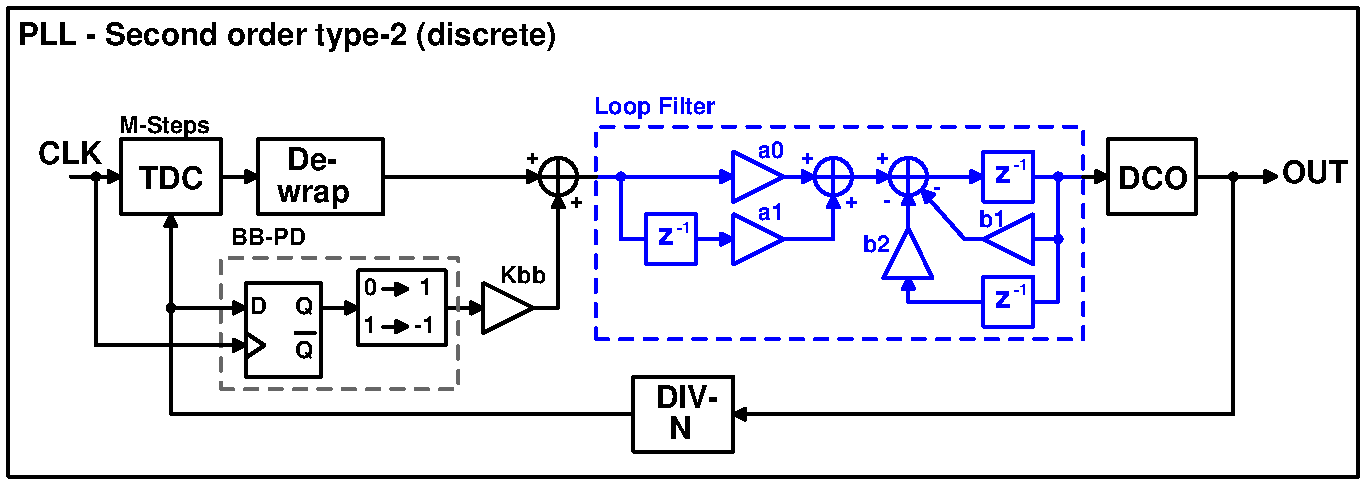
\includegraphics[width=0.8\textwidth, angle=0]{pll_sec_order_bb.pdf}

	\end{block}
		\begin{block}{Power Targets}
		\vspace{-.1em}
		\begin{table}[htb!]
			\tiny
			\centering
			\def\arraystretch{1.5}		
			\setlength\arrayrulewidth{0.75pt}
			\setlength{\tabcolsep}{1em} % for the horizontal padding
			\begin{tabular}{|l|l|l|l|l|}
				\hline 
				\rule[-1ex]{0pt}{2.5ex} \cellcolor{gray!40}\textbf{DCO} & \cellcolor{gray!40}\textbf{TDC} & \cellcolor{gray!40}\textbf{Divider }& \cellcolor{gray!40}\textbf{Other} & \cellcolor{gray!40}\textbf{SUM} \\ 
				\hline 
				\rule[-1ex]{0pt}{2.5ex} 70 $\mu$W& 20 $\mu$W & 10 $\mu$W & $<<$ 1 $\mu$W & 100 $\mu$W\\ 
				\hline 
			\end{tabular} 
			% \caption{Assigned specifications for branch line hybrid design.}
			% \label{asgn_specs}
		\end{table}   
	\end{block}

\end{frame}


% #############################################################################
% project phases
% #############################################################################


\begin{frame}
	\frametitle{Project Phases}
	\begin{block}{Autumn 2019}
		\footnotesize
		\begin{itemize}
			\item System modeling and simulation.
			\begin{itemize}
				\footnotesize
				\item Learn PLL theory in detail
				\item Evaluate feasability of PLL architectures (counter, TDC-based)
				\item Determine requirements for TDC/DCO/Divider/logic (bits of resolution, accuracy etc) to meet PLL performance specifications.
				\item Determine digital logic for loop filter, validate stability and lock time performance.
			\end{itemize}
			\item Research ultra-low power circuit topologies to implement system components that will meet determined requirements.
			\item Translate component-level specifications into schematic-level circuit designs.
			\begin{itemize}
				\footnotesize
				\item Try, fail, try again until functional at schematic level.
				\begin{itemize}
					\footnotesize
					\item I expect the TDC to be difficult.
				\end{itemize}
			\end{itemize}      
		\end{itemize}
	\end{block}
\end{frame}

% #############################################################################
% Project phases slide 2
% #############################################################################


\begin{frame}
	\frametitle{Project Phases (continued)}
	\begin{block}{Spring 2020}
		\begin{itemize}
			\footnotesize
			\item Finalize schematic-level design.
			\item Estabilish thorough tests for PLL performance (automated?) to help in layout.
			\item Layout of PLL.
			\begin{itemize}
				\footnotesize
				\item Design iteration until design specs met.
				\item Probably very time consuming.
			\end{itemize}
			\item Full characterization/validation of design performance. 
			\begin{itemize}
				\footnotesize
				\item Comprehensive Corners/Monte-Carlo testing (time consuming??)
				\item More design iteration if new issues crop up...
			\end{itemize}
			\item Thesis paper writing.
		\end{itemize}
	\end{block}
\end{frame}

% #############################################################################
% References
% #############################################################################


\begin{frame}
	\frametitle{References}
		\scriptsize
		[1] "Ultra-Low Power Wake-Up Receivers for Wireless Sensor Networks", N. Pletcher, J.M Rabaey, 2008.\\
		\hspace{16pt}\url{http://www.eecs.berkeley.edu/Pubs/TechRpts/2008/EECS-2008-59.html}\\
		\vspace{1em}
		% [2] "Minimum Achievable Phase Noise of RC Oscillators",
	% Navid et al. 2005
\end{frame}


\end{document}
